\section{System design}
\subsection{C4 model} \label{sec:ucdiagram}


This project adopts a structured approach to software architecture documentation based on the C4 model, a hierarchical visualization framework that enables clear communication of complex system architectures. The documentation is organized through four distinct levels of abstraction: software systems, containers, components, and code, each serving specific communication needs and technical depth requirements. The C4 model provides a lean graphical notation technique for modeling software system architectures through structural decomposition.
\begin{itemize}
    \item \textbf{Level 1 - Software Systems:} The highest level of abstraction describing systems that deliver value to users, whether human or automated. A software system represents something a single development team builds, owns, and has responsibility for, typically corresponding to team boundaries and deployment units.

    \item \textbf{Level 2 - Containers:} Runtime applications or data stores that must be running for the overall system to function. These include services, APIs, and message queues - essentially the major building blocks that distribute system responsibilities.

    \item \textbf{Level 3 - Components:} Internal elements within each container, showing how components interact with each other and external systems. This level reveals the logical groupings and interfaces that compose each container's functionality.

    \item \textbf{Level 4 - Code:} The most detailed view showing classes, interfaces, and code-level relationships.

\end{itemize}
This chapter will present and describe the C4 diagrams that have been developed.
\subsection{Level 1 - Software Systems}
\begin{figure}[H]
    \centering
    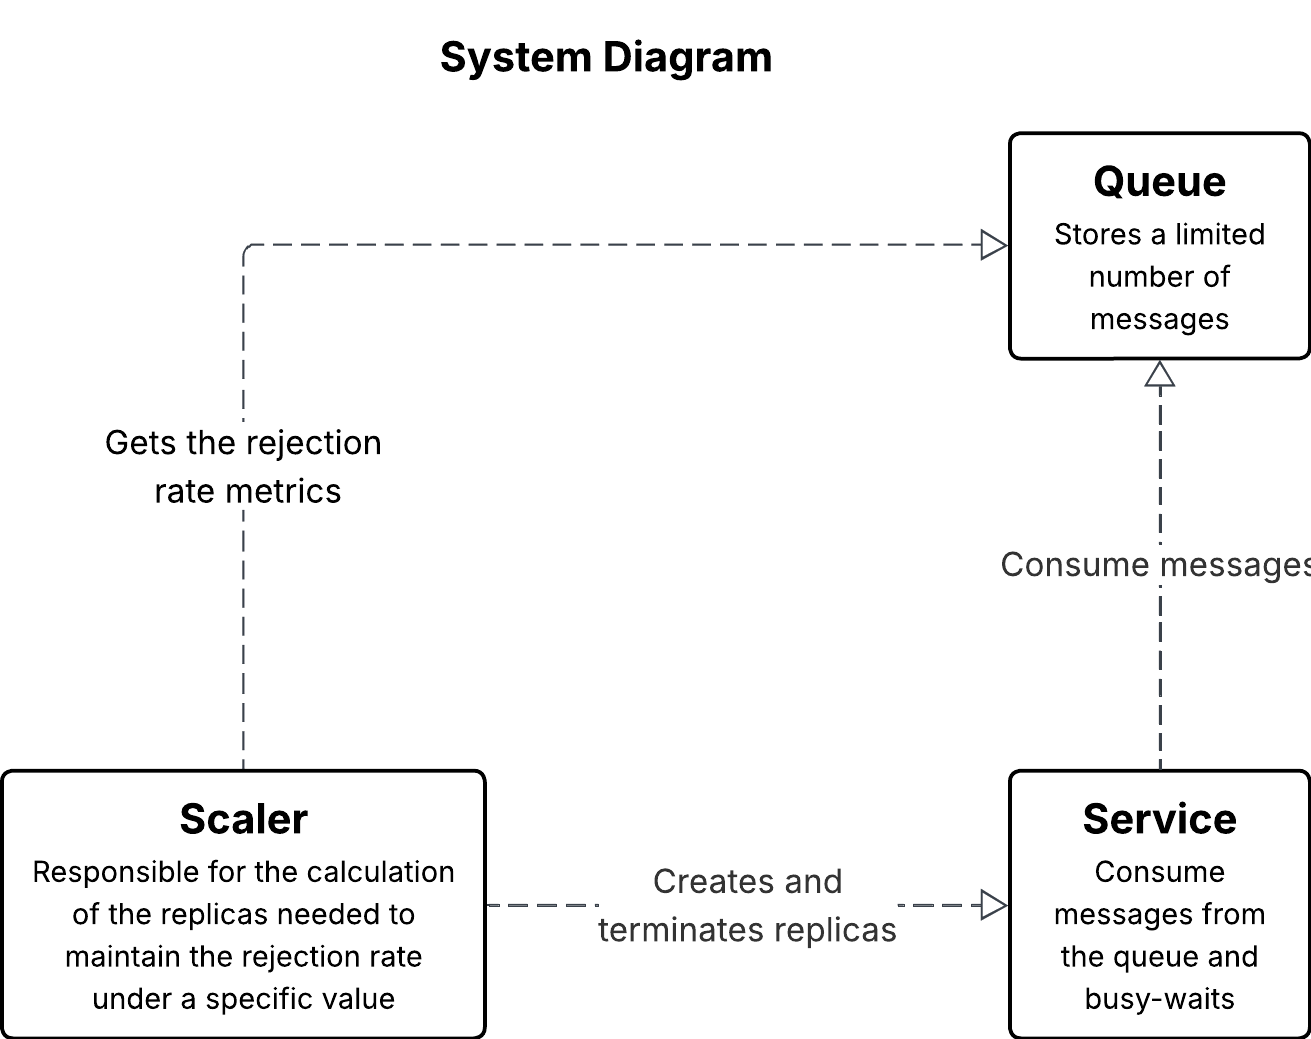
\includegraphics[width=0.75\linewidth]{images/C4 model/SystemDiagram.png}
    \caption{System Diagram}
    \label{fig:system_diagram}
\end{figure}

As shown in the Figure, the level 1 represents the highest level of abstraction of our system and it highlights its major components and functionalities. Its core comprehends a queue (reached by the messages generated) from which are exposed the necessary metrics to scale our service in order to achieve the chosen SLA. 

\subsection{Level 2 - Containers}

\begin{figure}[H]
    \centering
    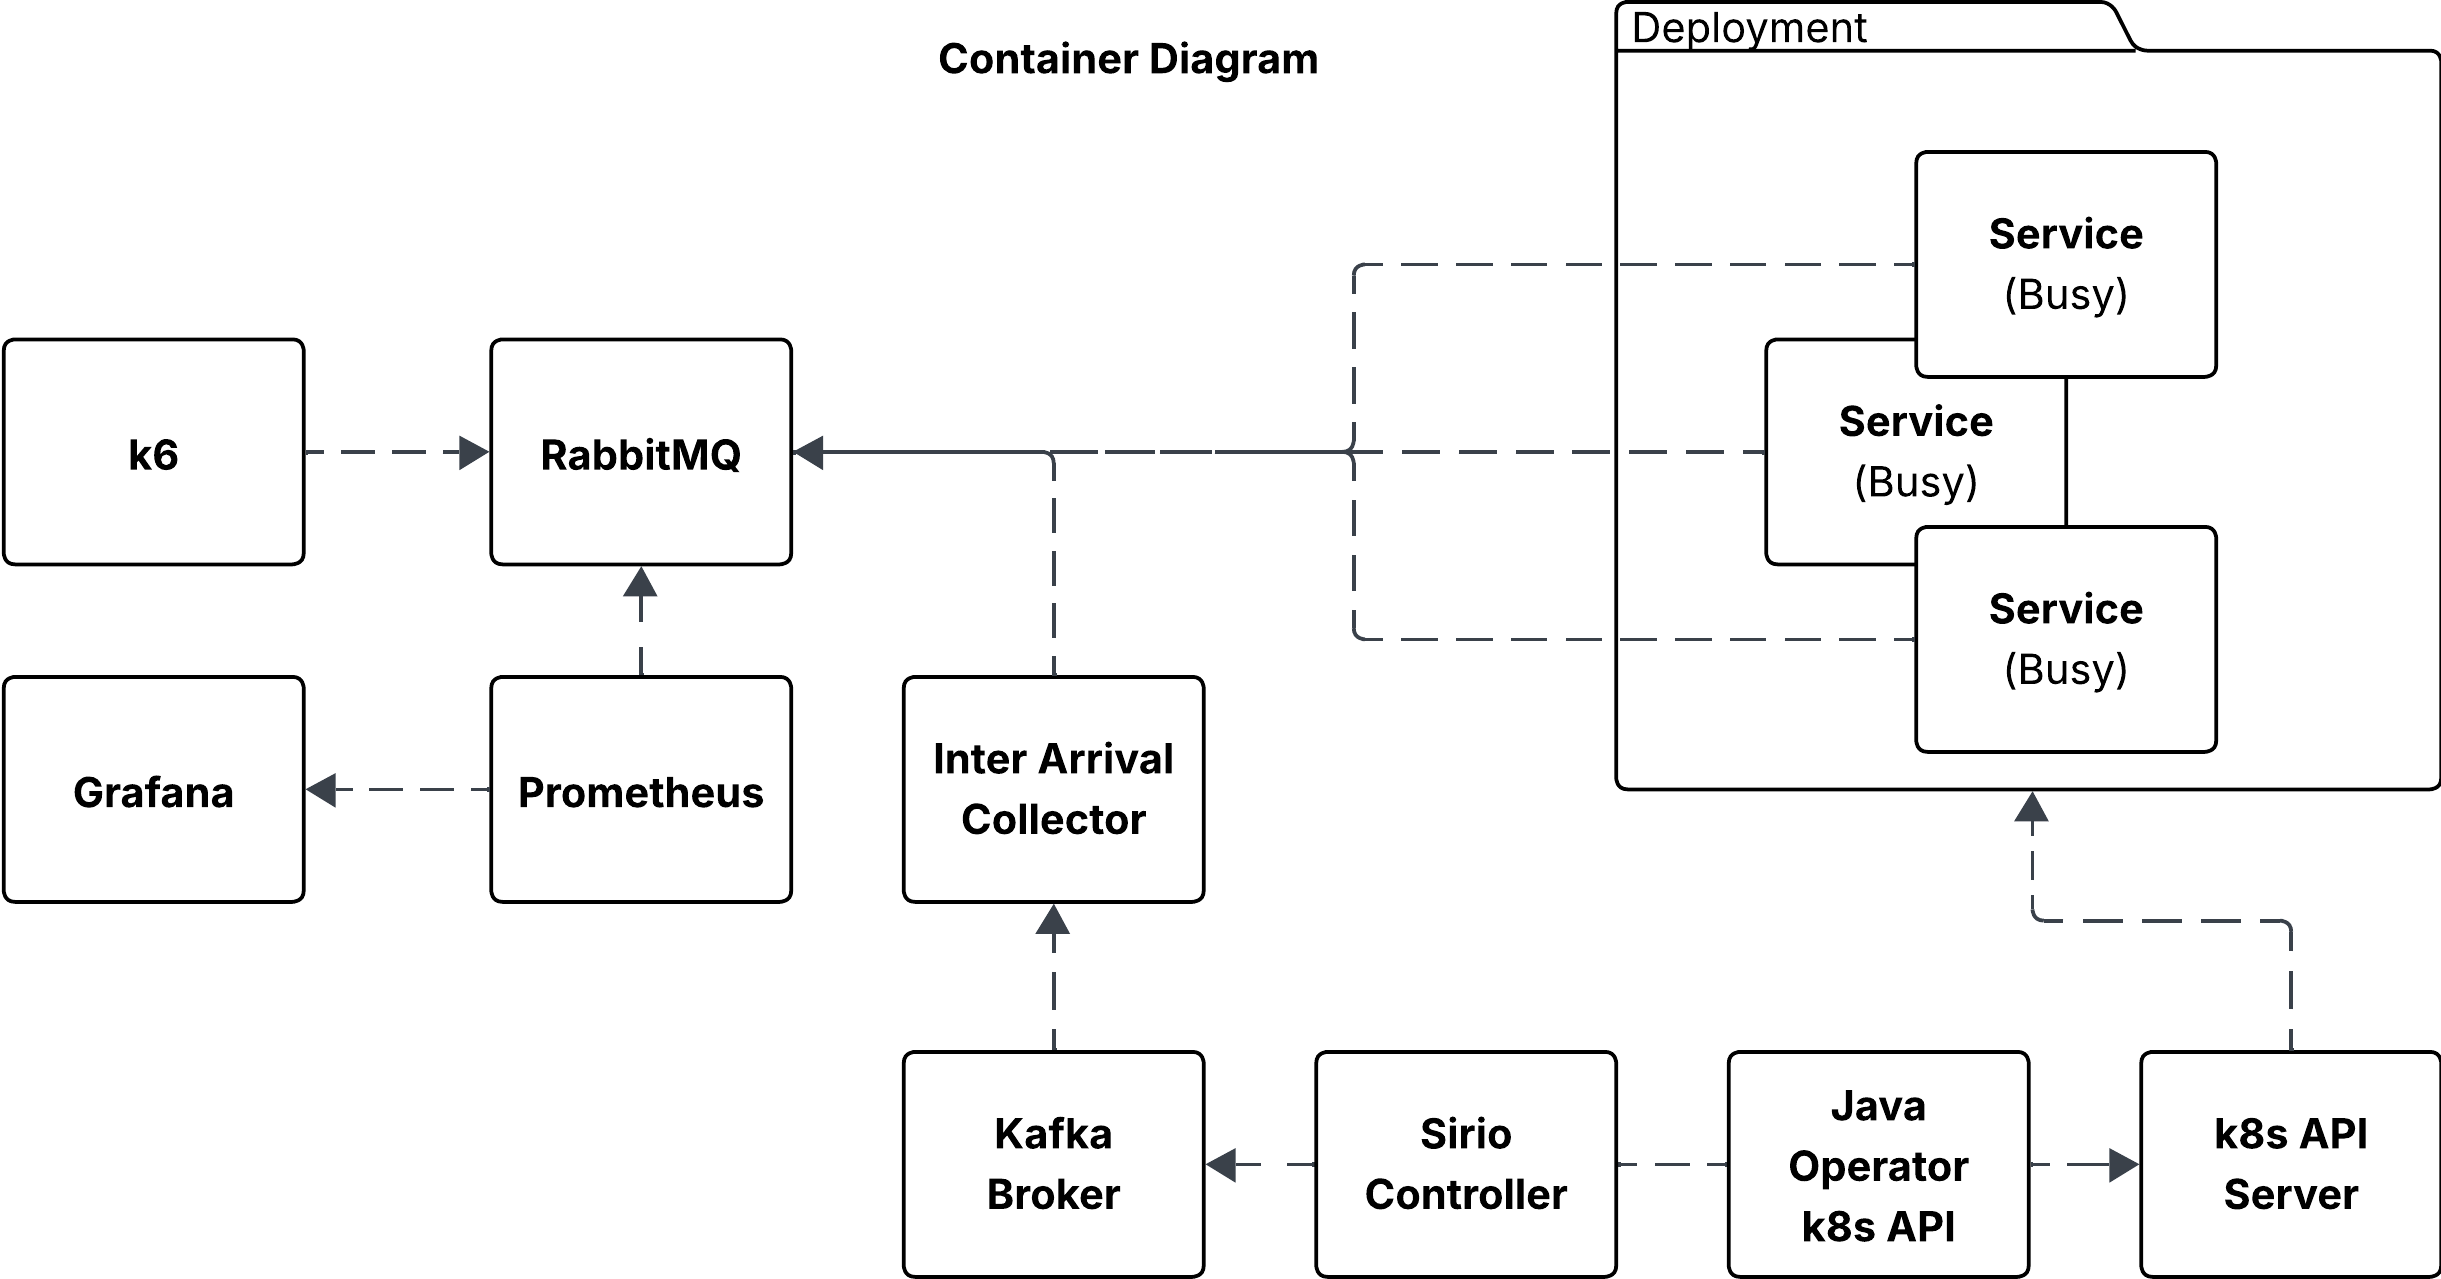
\includegraphics[width=0.75\linewidth]{images/C4 model/ContainerDiagram.png}
    \caption{Container Diagram}
    \label{fig:container_diagram}
\end{figure}


Going more in depth we see the container organization, which allows us to detail all the micro services built and their functions. Starting from left we have k6 to generate the load (in our case modeled as a state machine). The messages are stored in a RabbitMQ queue, which exposes the metrics of our interest on Grafana via Prometheus and to the Inter Arrival Collector. The Inter Arrival Collector exposes the CDF messages (with the CDF calculated on the interarrivals from the queue) on a Kafka broker that passes the messages to the Sirio Controller component, that uses the CDFs to estimate via the internal model the rejection rate. The number of replicas are estimated to keep the rejection rate under the target fixed. On the basis of this estimate, the kubernetes API is used to scale the services horizzontally (their number is increased or decreased).


\subsection{Level 3 - Components}
At the component architecture level, we have implemented a series of containers, entirely contained within the \verb|oris-predictive-autoscaler| namespace (ns). The architecture is divided into three main logical areas:
\begin{enumerate}
    \item The \textbf{System Under Test (SUT)}, which includes the custom applications and the basic messaging infrastructure (Kafka and RabbitMQ).
    \item The \textbf{Accessory Monitoring Services}, which provide observability and workload analysis capabilities.
    \item The \textbf{Security and Access Control (RBAC)} configuration, which governs the permissions of the various components within the cluster.
\end{enumerate}

\subsubsection{System Under Test (SUT)}
The SUT represents the core of the system and includes both the custom-developed application components (yellow background) and the infrastructure services they rely on (white background).
Asynchronous communication and data flow management are handled by two message brokering systems:
\begin{itemize}
\item \textbf{rabbitmq}: The message broker, used as the incoming request queue for the service. It is also implemented as a \textbf{StatefulSet (sts)} and configured via two \textbf{ConfigMaps (cm)}: \verb|rabbitmq-definitions| and \verb|rabbitmq-config|, which define its policies, queues, and initial settings. A \textbf{Service (svc)} ensures its accessibility.
    \item \textbf{kafka}: Used as a notification and data exchange system between the \verb|inter-arrival-collector| and the \verb|sirio-controller|. Being a stateful system, it is implemented as a \textbf{StatefulSet (sts)} to ensure stable network identities and persistent storage, managed via a \textbf{PersistentVolumeClaim (pvc)}. A \textbf{Service (svc)} exposes Kafka within the cluster, allowing components to communicate with it.

\end{itemize}

\subsubsection{Custom Services}
These are the components where the specific business logic of the autoscaling system resides.
\begin{itemize}
    \item \textbf{sirio-controller}: Contains the \verb|sirio-controller| \textbf{Deployment}, which represents the brain of the system. This controller implements the predictive autoscaling logic, monitoring metrics and making decisions on how and when to scale the service. The deployment's code diagram will be presented in the next chapter, \ref{sec:code}.
    \item \textbf{inter-arrival-collector}: This \textbf{Deployment} is responsible for collecting the inter-arrival times of requests. Acquiring this data is fundamental for the predictive model. Once collected, the data is sent to Kafka to be processed by the \verb|sirio-controller|.
    \item \textbf{python-service}: This \textbf{Deployment} represents the target application, i.e., the service that is monitored and whose number of replicas is dynamically managed by the \verb|sirio-controller|.
\end{itemize}

\subsubsection{Operations and Monitoring}
These services (green background) are not part of the main application logic (SUT) but are crucial for collecting metrics, analyzing performance, and visualizing the system's state.

\begin{itemize}
    \item \textbf{prometheus}: It is the central monitoring and alerting system. Implemented as a \textbf{Deployment}, it uses a \textbf{ConfigMap} (\verb|prometheus-config|) to define the targets from which to scrape metrics (such as \verb|kube-state-metrics| and the SUT applications). A \textbf{Service} exposes its interface so that it can be easily reached by Grafana.
    \item \textbf{kube-state-metrics}: An essential service that connects to the Kubernetes API Server to generate metrics about the state of cluster objects (in this case, the number of pods in a deployment). These metrics are then collected by Prometheus to be displayed on Grafana.
    \item \textbf{grafana}: A visualization tool that connects to Prometheus as a datasource. Its \textbf{Deployment} is configured via two \textbf{ConfigMaps}: \verb|grafana-datasource| to set up the connection to Prometheus and \verb|grafana-dashboards| to preload custom dashboards. 
\end{itemize}

 \begin{figure}[ht]
    \centering
    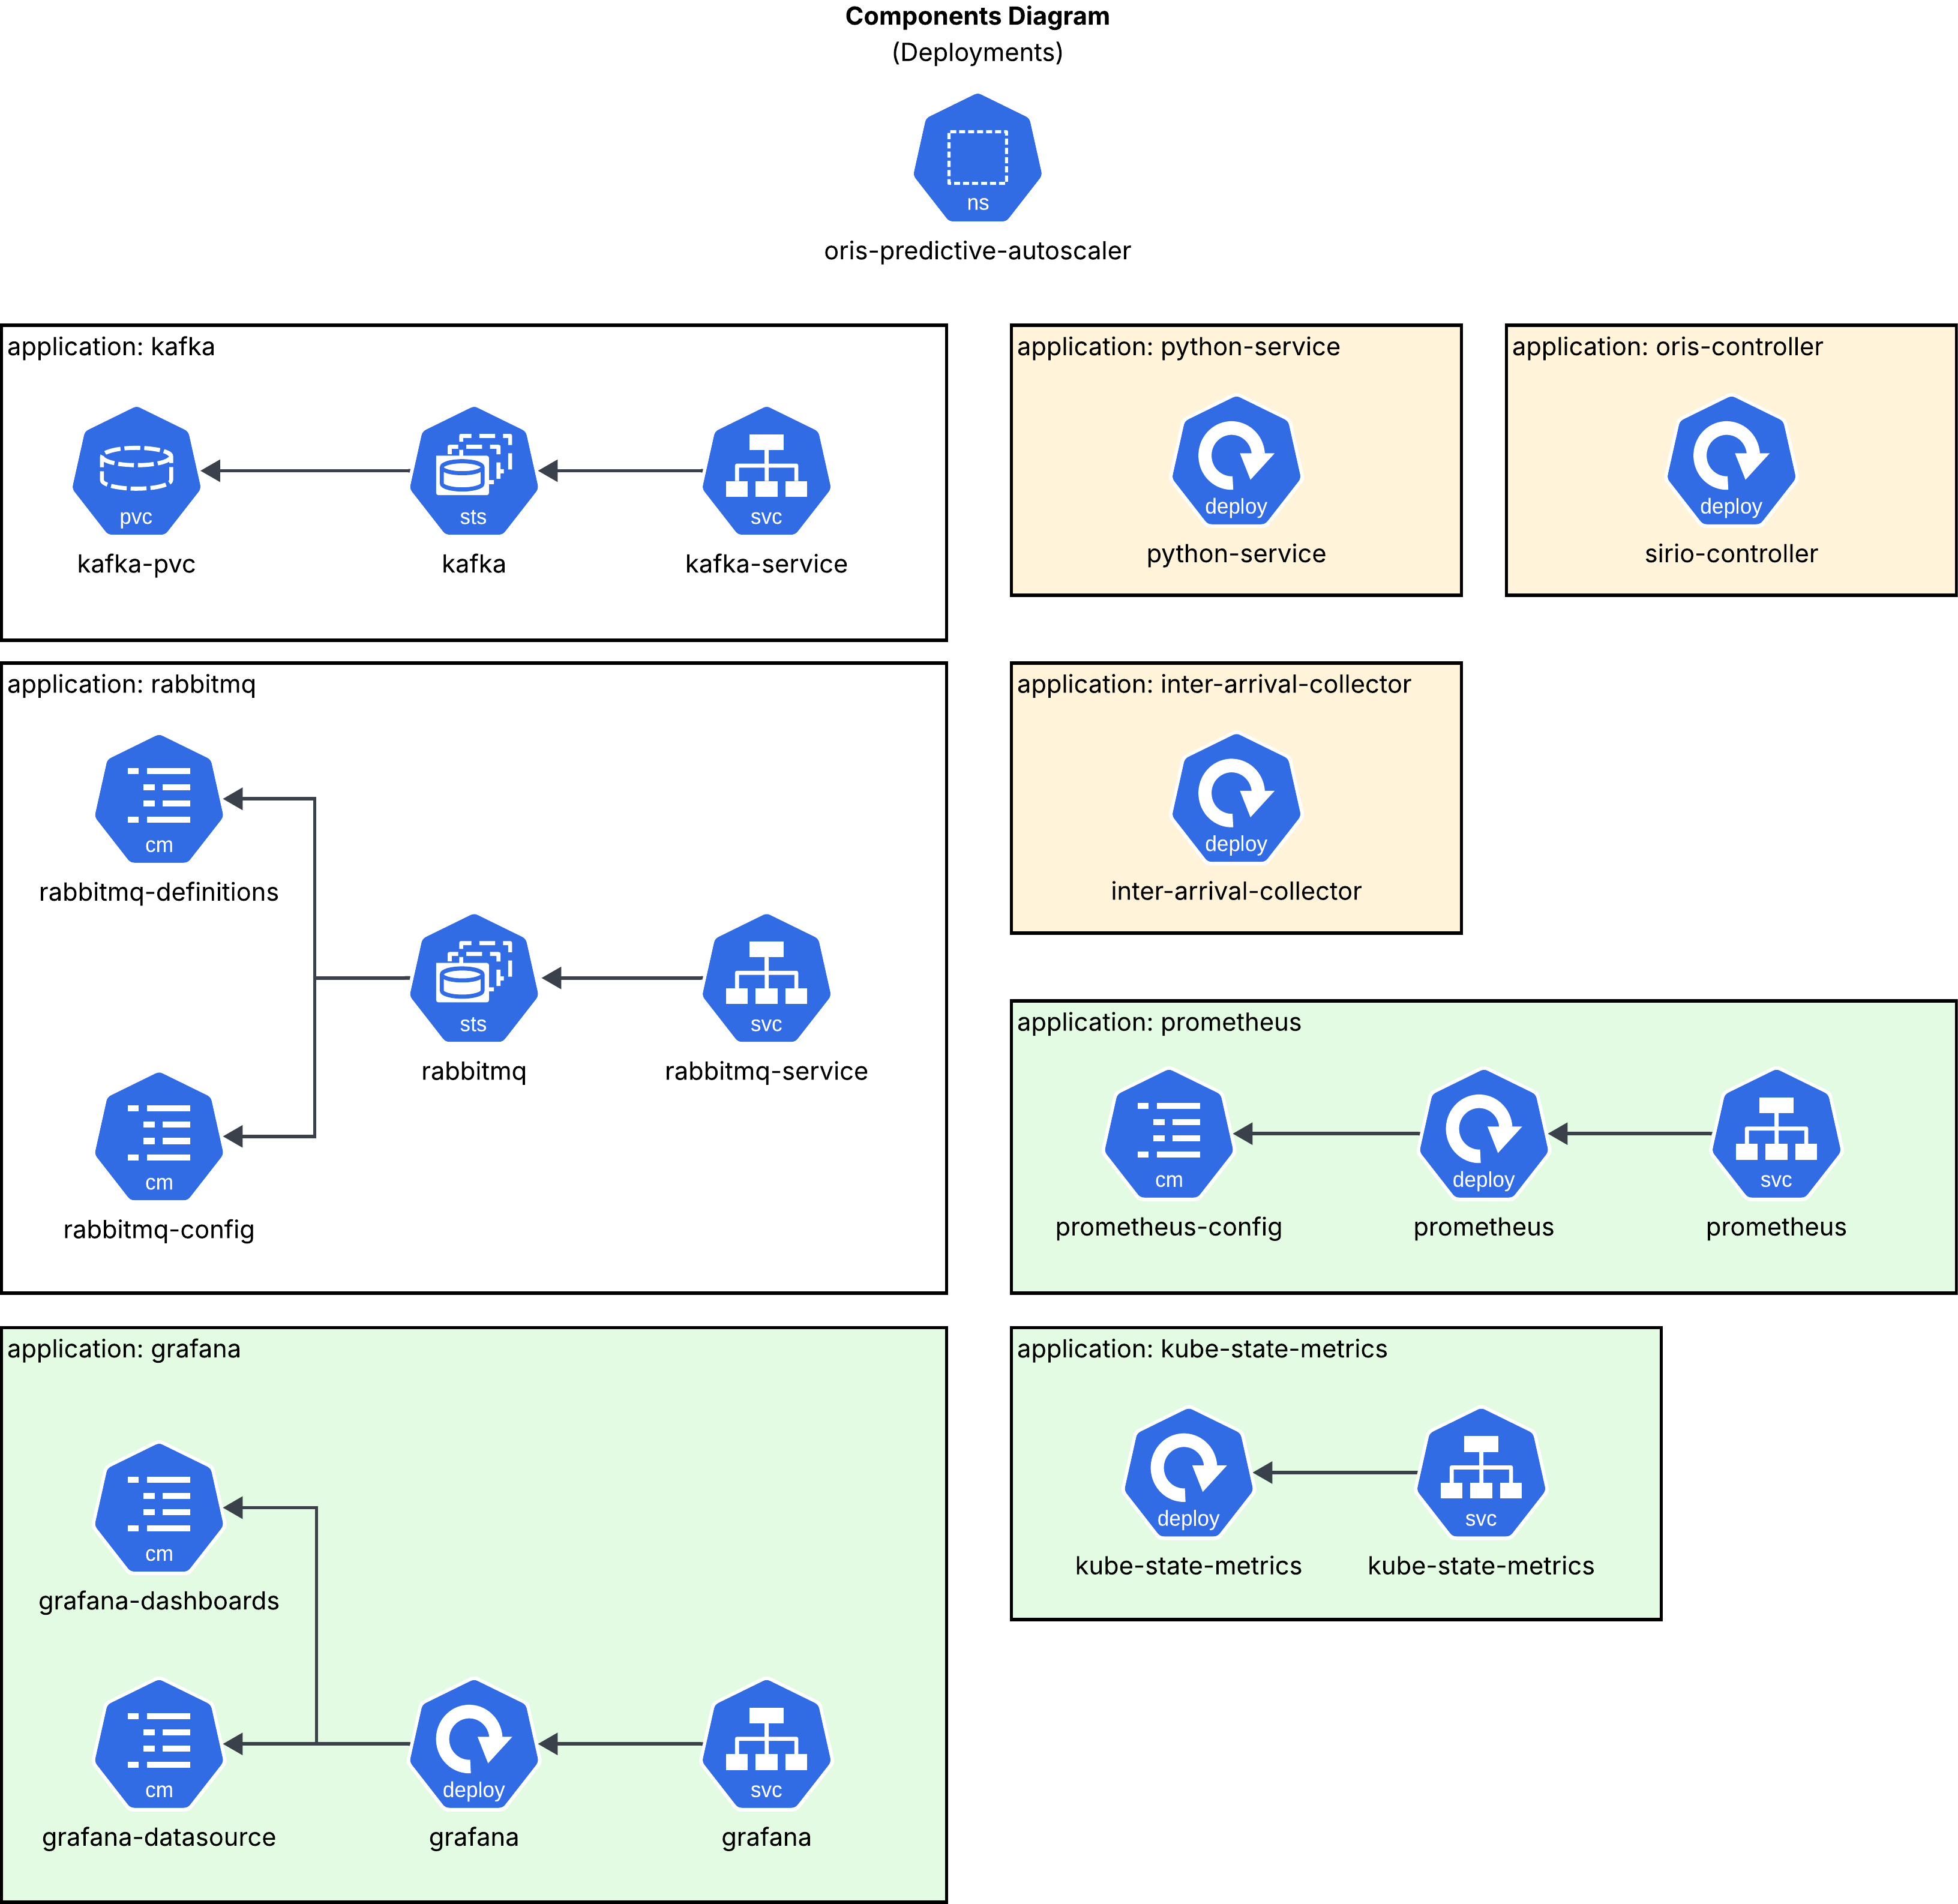
\includegraphics[width=0.75\linewidth]{images/C4 model/componentDiagram_deploy.png}
    \caption{Deployments Diagram}
    \label{fig:component_diagram_deploy}
\end{figure}

\subsubsection{Role-Based Access Control}
 The second diagram illustrates the RBAC (Role-Based Access Control) configurations that ensure each component operates on the principle of least privilege, accessing only the resources that are strictly necessary.

\begin{itemize}
    \item \textbf{kube-state-metrics-rbac}: In order to generate metrics on the entire cluster, this service needs read permissions on all Kubernetes objects. Its configuration includes:
    \begin{itemize}
        \item A \textbf{ServiceAccount (sa)}: \verb|kube-state-metrics|, the identity used by the pod.
        \item A \textbf{ClusterRole (c.role)}: Defines \verb|get|, \verb|list|, \verb|watch| permissions at the cluster level.
        \item A \textbf{ClusterRoleBinding (crb)}: Binds the \verb|ClusterRole| to the \verb|ServiceAccount|, making the permissions effective.
    \end{itemize}
    \item \textbf{sirio-controller-rbac}: Being the heart of the autoscaling logic, the controller must be able to monitor and modify the state of other objects (like Deployments). In this case as well, the configuration uses a \textbf{ServiceAccount}, a \textbf{ClusterRole}, and a \textbf{ClusterRoleBinding} to grant it the necessary permissions to operate at the cluster scale.
    \item \textbf{prometheus-operator-rbac}: This is the most complex configuration because it deals with defining the functionalities and permissions of the Prometheus Operator. The operator requires permissions at both the namespace and cluster levels:
    \begin{itemize}
        \item A \textbf{Role} and a \textbf{RoleBinding (rb)}: grant it specific permissions within the \verb|oris-predictive-autoscaler| namespace.
        \item A \textbf{ClusterRole} and a \textbf{ClusterRoleBinding (crb)}: grant it broader permissions, necessary to discover services to monitor across the entire cluster or to manage resources globally.
    \end{itemize}
\end{itemize}

\begin{figure}[ht]
    \centering
    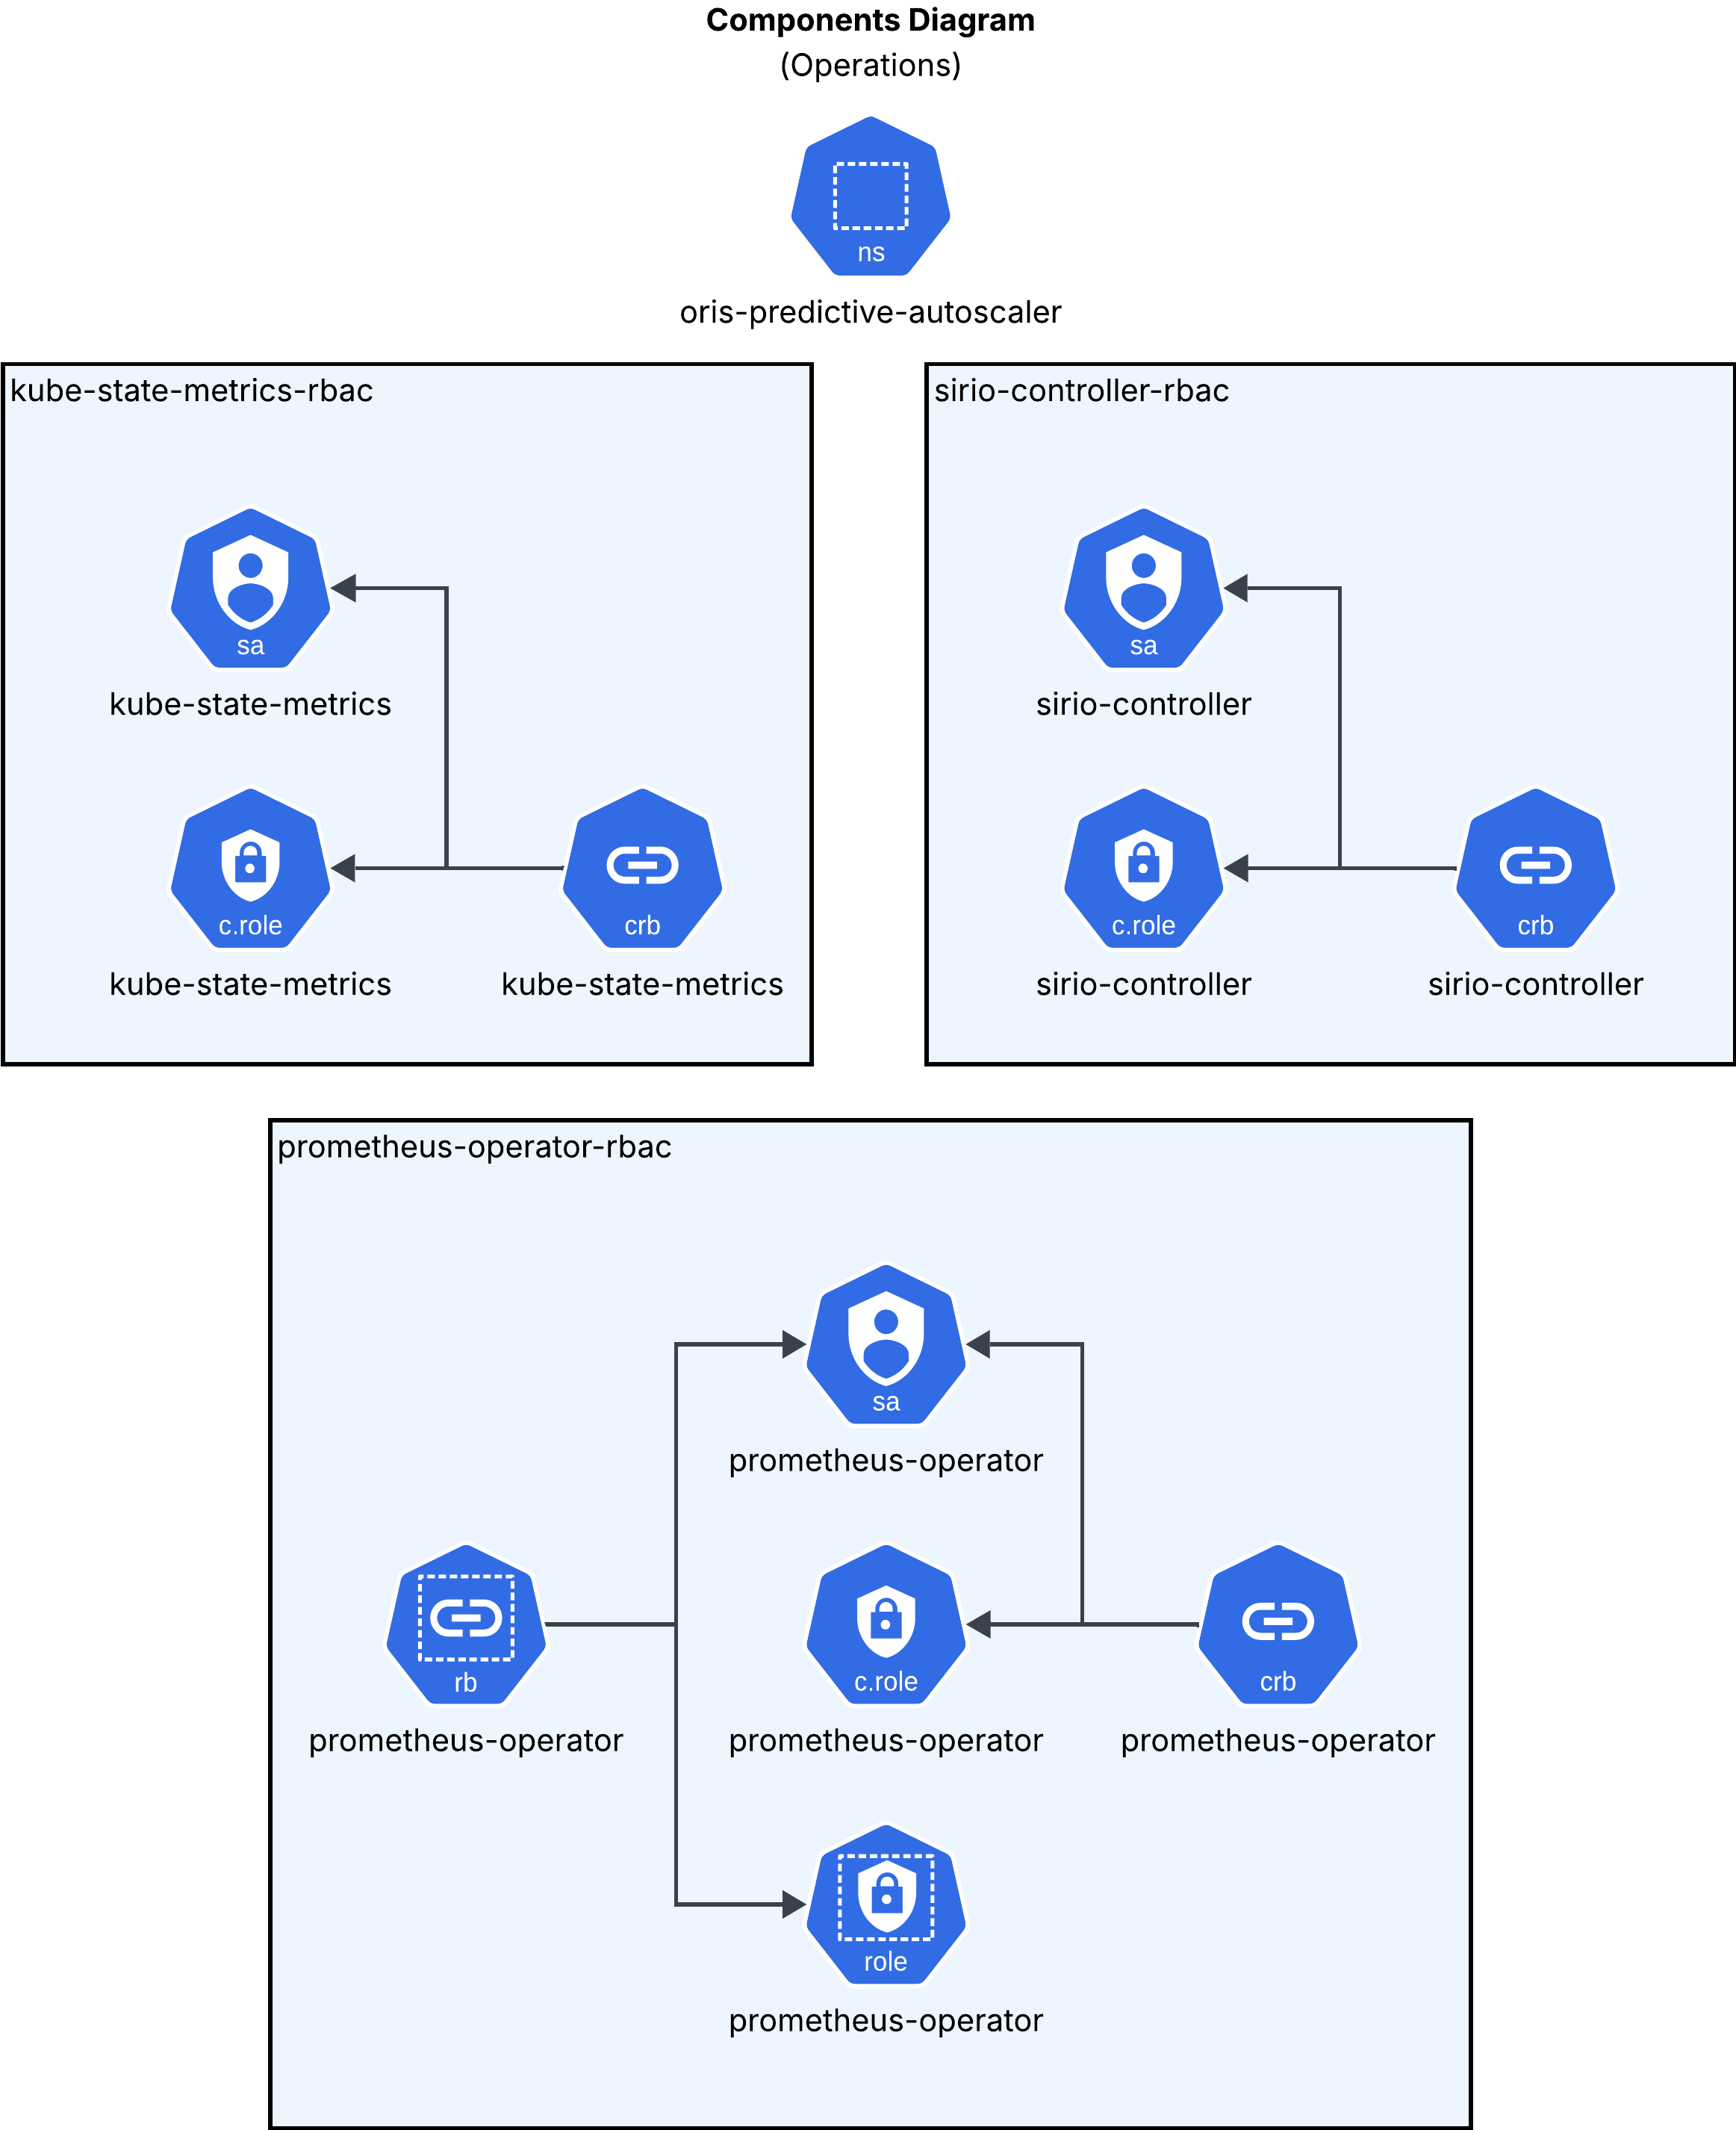
\includegraphics[width=0.75\linewidth]{images/C4 model/componentDiagram_operations.png}
    \caption{Operations Diagram}
    \label{fig:uccomponent_diagram_operations}
\end{figure}
\newpage
\subsection{Level 4 - Code} \label{sec:code}
And finally, the code:

\begin{figure}[H]
    \centering
    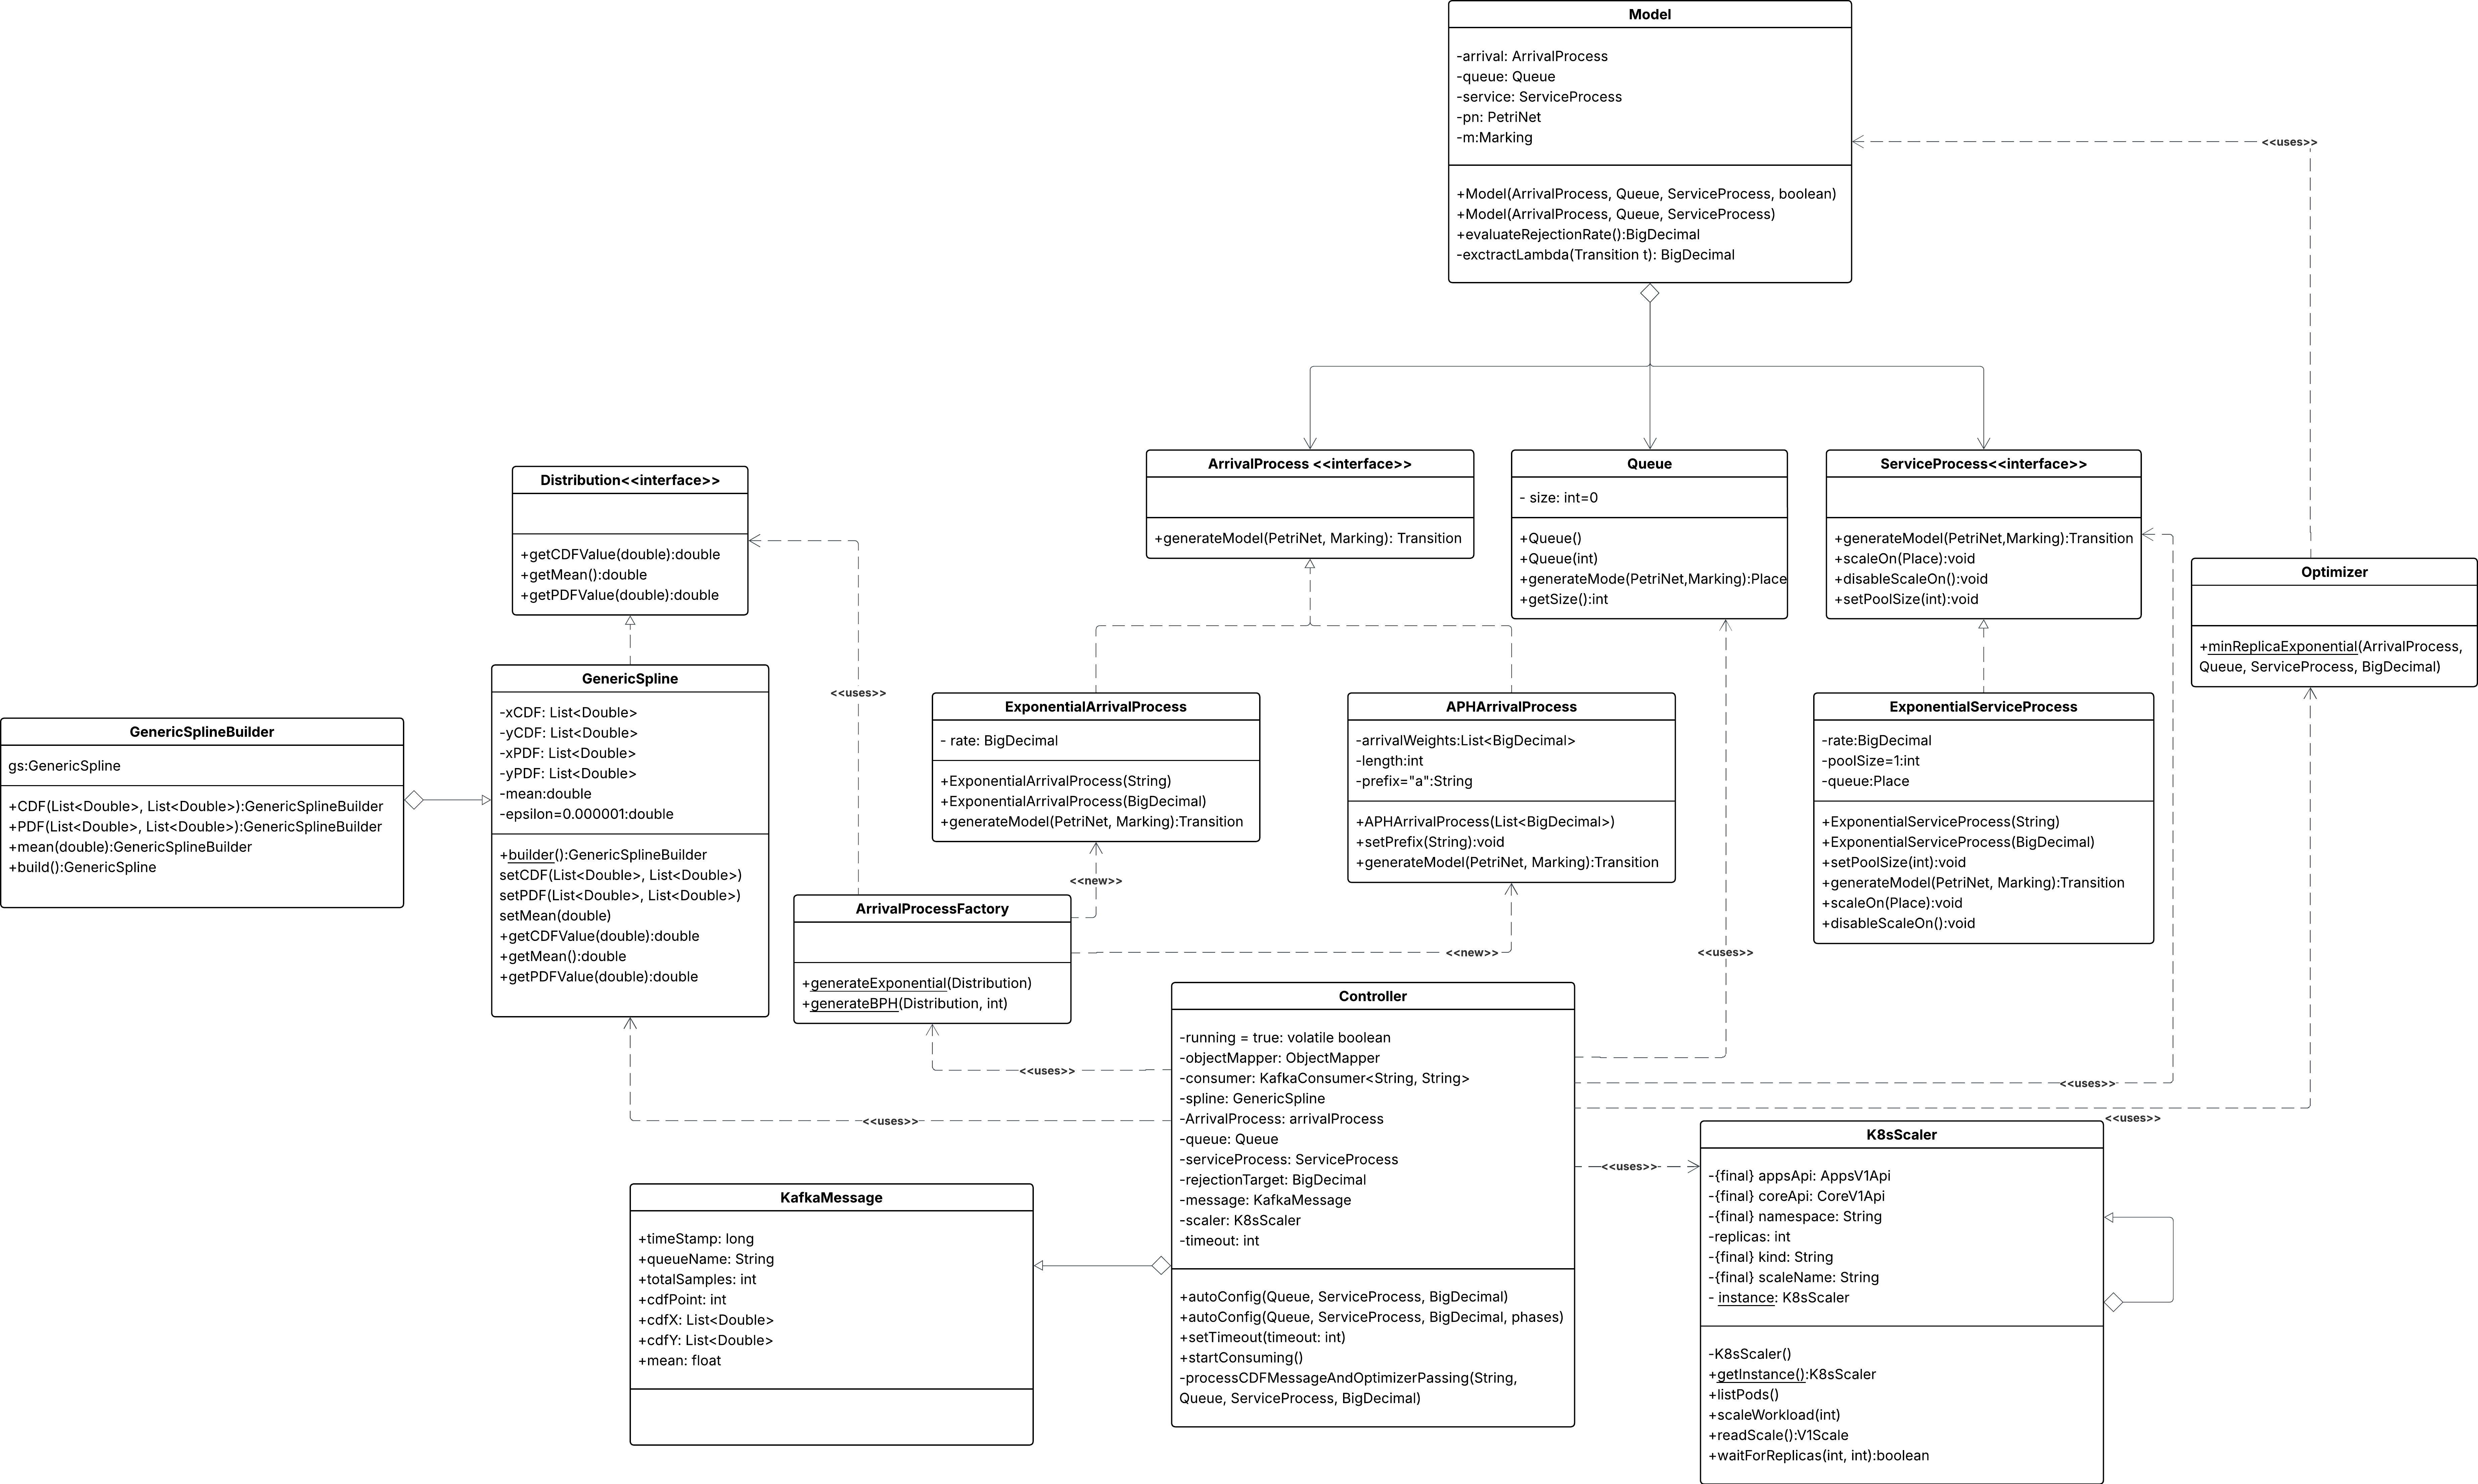
\includegraphics[width=1\linewidth]{images/C4 model/UML.png}
    \caption{UML Class Diagram}
    \label{fig:uml_diagram}
\end{figure}

This is the UML class diagram for the Sirio controller. What is good to note is that it is the piece of code to construct the model and evaluate the rejection rate constructing a real model of the problem and using the CDF received and mapped in the KafkaMessage class. All things considered, the core of this code is the optimizer because it uses all the other elements to iteratively evaluate the rejection rate for an increasing number of replicas. When the best number is found, the scaler is commanded. Follow \href{https://lucid.app/lucidchart/5c1b70c3-c1c8-470e-b04a-fefab525a1fc/edit?invitationId=inv_05163187-b3ea-4a1a-a14b-3cdabad1d3d5&page=XRAN4fSOEXo6#}{this link} for a better visualization.